\documentclass{article} % For LaTeX2e
\usepackage{iclr2022_conference,times}
\usepackage{tabularx}
\usepackage{array}
\usepackage{caption}
\usepackage{booktabs}
\usepackage[table]{xcolor}
\usepackage{makecell}
\usepackage{hyperref}
\usepackage{url}
\usepackage{graphicx}
\usepackage{gensymb}
% Optional math commands from https://github.com/goodfeli/dlbook_notation.
%%%%% NEW MATH DEFINITIONS %%%%%

\usepackage{amsmath,amsfonts,bm}

% Mark sections of captions for referring to divisions of figures
\newcommand{\figleft}{{\em (Left)}}
\newcommand{\figcenter}{{\em (Center)}}
\newcommand{\figright}{{\em (Right)}}
\newcommand{\figtop}{{\em (Top)}}
\newcommand{\figbottom}{{\em (Bottom)}}
\newcommand{\captiona}{{\em (a)}}
\newcommand{\captionb}{{\em (b)}}
\newcommand{\captionc}{{\em (c)}}
\newcommand{\captiond}{{\em (d)}}

% Highlight a newly defined term
\newcommand{\newterm}[1]{{\bf #1}}


% Figure reference, lower-case.
\def\figref#1{figure~\ref{#1}}
% Figure reference, capital. For start of sentence
\def\Figref#1{Figure~\ref{#1}}
\def\twofigref#1#2{figures \ref{#1} and \ref{#2}}
\def\quadfigref#1#2#3#4{figures \ref{#1}, \ref{#2}, \ref{#3} and \ref{#4}}
% Section reference, lower-case.
\def\secref#1{section~\ref{#1}}
% Section reference, capital.
\def\Secref#1{Section~\ref{#1}}
% Reference to two sections.
\def\twosecrefs#1#2{sections \ref{#1} and \ref{#2}}
% Reference to three sections.
\def\secrefs#1#2#3{sections \ref{#1}, \ref{#2} and \ref{#3}}
% Reference to an equation, lower-case.
\def\eqref#1{equation~\ref{#1}}
% Reference to an equation, upper case
\def\Eqref#1{Equation~\ref{#1}}
% A raw reference to an equation---avoid using if possible
\def\plaineqref#1{\ref{#1}}
% Reference to a chapter, lower-case.
\def\chapref#1{chapter~\ref{#1}}
% Reference to an equation, upper case.
\def\Chapref#1{Chapter~\ref{#1}}
% Reference to a range of chapters
\def\rangechapref#1#2{chapters\ref{#1}--\ref{#2}}
% Reference to an algorithm, lower-case.
\def\algref#1{algorithm~\ref{#1}}
% Reference to an algorithm, upper case.
\def\Algref#1{Algorithm~\ref{#1}}
\def\twoalgref#1#2{algorithms \ref{#1} and \ref{#2}}
\def\Twoalgref#1#2{Algorithms \ref{#1} and \ref{#2}}
% Reference to a part, lower case
\def\partref#1{part~\ref{#1}}
% Reference to a part, upper case
\def\Partref#1{Part~\ref{#1}}
\def\twopartref#1#2{parts \ref{#1} and \ref{#2}}

\def\ceil#1{\lceil #1 \rceil}
\def\floor#1{\lfloor #1 \rfloor}
\def\1{\bm{1}}
\newcommand{\train}{\mathcal{D}}
\newcommand{\valid}{\mathcal{D_{\mathrm{valid}}}}
\newcommand{\test}{\mathcal{D_{\mathrm{test}}}}

\def\eps{{\epsilon}}


% Random variables
\def\reta{{\textnormal{$\eta$}}}
\def\ra{{\textnormal{a}}}
\def\rb{{\textnormal{b}}}
\def\rc{{\textnormal{c}}}
\def\rd{{\textnormal{d}}}
\def\re{{\textnormal{e}}}
\def\rf{{\textnormal{f}}}
\def\rg{{\textnormal{g}}}
\def\rh{{\textnormal{h}}}
\def\ri{{\textnormal{i}}}
\def\rj{{\textnormal{j}}}
\def\rk{{\textnormal{k}}}
\def\rl{{\textnormal{l}}}
% rm is already a command, just don't name any random variables m
\def\rn{{\textnormal{n}}}
\def\ro{{\textnormal{o}}}
\def\rp{{\textnormal{p}}}
\def\rq{{\textnormal{q}}}
\def\rr{{\textnormal{r}}}
\def\rs{{\textnormal{s}}}
\def\rt{{\textnormal{t}}}
\def\ru{{\textnormal{u}}}
\def\rv{{\textnormal{v}}}
\def\rw{{\textnormal{w}}}
\def\rx{{\textnormal{x}}}
\def\ry{{\textnormal{y}}}
\def\rz{{\textnormal{z}}}

% Random vectors
\def\rvepsilon{{\mathbf{\epsilon}}}
\def\rvtheta{{\mathbf{\theta}}}
\def\rva{{\mathbf{a}}}
\def\rvb{{\mathbf{b}}}
\def\rvc{{\mathbf{c}}}
\def\rvd{{\mathbf{d}}}
\def\rve{{\mathbf{e}}}
\def\rvf{{\mathbf{f}}}
\def\rvg{{\mathbf{g}}}
\def\rvh{{\mathbf{h}}}
\def\rvu{{\mathbf{i}}}
\def\rvj{{\mathbf{j}}}
\def\rvk{{\mathbf{k}}}
\def\rvl{{\mathbf{l}}}
\def\rvm{{\mathbf{m}}}
\def\rvn{{\mathbf{n}}}
\def\rvo{{\mathbf{o}}}
\def\rvp{{\mathbf{p}}}
\def\rvq{{\mathbf{q}}}
\def\rvr{{\mathbf{r}}}
\def\rvs{{\mathbf{s}}}
\def\rvt{{\mathbf{t}}}
\def\rvu{{\mathbf{u}}}
\def\rvv{{\mathbf{v}}}
\def\rvw{{\mathbf{w}}}
\def\rvx{{\mathbf{x}}}
\def\rvy{{\mathbf{y}}}
\def\rvz{{\mathbf{z}}}

% Elements of random vectors
\def\erva{{\textnormal{a}}}
\def\ervb{{\textnormal{b}}}
\def\ervc{{\textnormal{c}}}
\def\ervd{{\textnormal{d}}}
\def\erve{{\textnormal{e}}}
\def\ervf{{\textnormal{f}}}
\def\ervg{{\textnormal{g}}}
\def\ervh{{\textnormal{h}}}
\def\ervi{{\textnormal{i}}}
\def\ervj{{\textnormal{j}}}
\def\ervk{{\textnormal{k}}}
\def\ervl{{\textnormal{l}}}
\def\ervm{{\textnormal{m}}}
\def\ervn{{\textnormal{n}}}
\def\ervo{{\textnormal{o}}}
\def\ervp{{\textnormal{p}}}
\def\ervq{{\textnormal{q}}}
\def\ervr{{\textnormal{r}}}
\def\ervs{{\textnormal{s}}}
\def\ervt{{\textnormal{t}}}
\def\ervu{{\textnormal{u}}}
\def\ervv{{\textnormal{v}}}
\def\ervw{{\textnormal{w}}}
\def\ervx{{\textnormal{x}}}
\def\ervy{{\textnormal{y}}}
\def\ervz{{\textnormal{z}}}

% Random matrices
\def\rmA{{\mathbf{A}}}
\def\rmB{{\mathbf{B}}}
\def\rmC{{\mathbf{C}}}
\def\rmD{{\mathbf{D}}}
\def\rmE{{\mathbf{E}}}
\def\rmF{{\mathbf{F}}}
\def\rmG{{\mathbf{G}}}
\def\rmH{{\mathbf{H}}}
\def\rmI{{\mathbf{I}}}
\def\rmJ{{\mathbf{J}}}
\def\rmK{{\mathbf{K}}}
\def\rmL{{\mathbf{L}}}
\def\rmM{{\mathbf{M}}}
\def\rmN{{\mathbf{N}}}
\def\rmO{{\mathbf{O}}}
\def\rmP{{\mathbf{P}}}
\def\rmQ{{\mathbf{Q}}}
\def\rmR{{\mathbf{R}}}
\def\rmS{{\mathbf{S}}}
\def\rmT{{\mathbf{T}}}
\def\rmU{{\mathbf{U}}}
\def\rmV{{\mathbf{V}}}
\def\rmW{{\mathbf{W}}}
\def\rmX{{\mathbf{X}}}
\def\rmY{{\mathbf{Y}}}
\def\rmZ{{\mathbf{Z}}}

% Elements of random matrices
\def\ermA{{\textnormal{A}}}
\def\ermB{{\textnormal{B}}}
\def\ermC{{\textnormal{C}}}
\def\ermD{{\textnormal{D}}}
\def\ermE{{\textnormal{E}}}
\def\ermF{{\textnormal{F}}}
\def\ermG{{\textnormal{G}}}
\def\ermH{{\textnormal{H}}}
\def\ermI{{\textnormal{I}}}
\def\ermJ{{\textnormal{J}}}
\def\ermK{{\textnormal{K}}}
\def\ermL{{\textnormal{L}}}
\def\ermM{{\textnormal{M}}}
\def\ermN{{\textnormal{N}}}
\def\ermO{{\textnormal{O}}}
\def\ermP{{\textnormal{P}}}
\def\ermQ{{\textnormal{Q}}}
\def\ermR{{\textnormal{R}}}
\def\ermS{{\textnormal{S}}}
\def\ermT{{\textnormal{T}}}
\def\ermU{{\textnormal{U}}}
\def\ermV{{\textnormal{V}}}
\def\ermW{{\textnormal{W}}}
\def\ermX{{\textnormal{X}}}
\def\ermY{{\textnormal{Y}}}
\def\ermZ{{\textnormal{Z}}}

% Vectors
\def\vzero{{\bm{0}}}
\def\vone{{\bm{1}}}
\def\vmu{{\bm{\mu}}}
\def\vtheta{{\bm{\theta}}}
\def\va{{\bm{a}}}
\def\vb{{\bm{b}}}
\def\vc{{\bm{c}}}
\def\vd{{\bm{d}}}
\def\ve{{\bm{e}}}
\def\vf{{\bm{f}}}
\def\vg{{\bm{g}}}
\def\vh{{\bm{h}}}
\def\vi{{\bm{i}}}
\def\vj{{\bm{j}}}
\def\vk{{\bm{k}}}
\def\vl{{\bm{l}}}
\def\vm{{\bm{m}}}
\def\vn{{\bm{n}}}
\def\vo{{\bm{o}}}
\def\vp{{\bm{p}}}
\def\vq{{\bm{q}}}
\def\vr{{\bm{r}}}
\def\vs{{\bm{s}}}
\def\vt{{\bm{t}}}
\def\vu{{\bm{u}}}
\def\vv{{\bm{v}}}
\def\vw{{\bm{w}}}
\def\vx{{\bm{x}}}
\def\vy{{\bm{y}}}
\def\vz{{\bm{z}}}

% Elements of vectors
\def\evalpha{{\alpha}}
\def\evbeta{{\beta}}
\def\evepsilon{{\epsilon}}
\def\evlambda{{\lambda}}
\def\evomega{{\omega}}
\def\evmu{{\mu}}
\def\evpsi{{\psi}}
\def\evsigma{{\sigma}}
\def\evtheta{{\theta}}
\def\eva{{a}}
\def\evb{{b}}
\def\evc{{c}}
\def\evd{{d}}
\def\eve{{e}}
\def\evf{{f}}
\def\evg{{g}}
\def\evh{{h}}
\def\evi{{i}}
\def\evj{{j}}
\def\evk{{k}}
\def\evl{{l}}
\def\evm{{m}}
\def\evn{{n}}
\def\evo{{o}}
\def\evp{{p}}
\def\evq{{q}}
\def\evr{{r}}
\def\evs{{s}}
\def\evt{{t}}
\def\evu{{u}}
\def\evv{{v}}
\def\evw{{w}}
\def\evx{{x}}
\def\evy{{y}}
\def\evz{{z}}

% Matrix
\def\mA{{\bm{A}}}
\def\mB{{\bm{B}}}
\def\mC{{\bm{C}}}
\def\mD{{\bm{D}}}
\def\mE{{\bm{E}}}
\def\mF{{\bm{F}}}
\def\mG{{\bm{G}}}
\def\mH{{\bm{H}}}
\def\mI{{\bm{I}}}
\def\mJ{{\bm{J}}}
\def\mK{{\bm{K}}}
\def\mL{{\bm{L}}}
\def\mM{{\bm{M}}}
\def\mN{{\bm{N}}}
\def\mO{{\bm{O}}}
\def\mP{{\bm{P}}}
\def\mQ{{\bm{Q}}}
\def\mR{{\bm{R}}}
\def\mS{{\bm{S}}}
\def\mT{{\bm{T}}}
\def\mU{{\bm{U}}}
\def\mV{{\bm{V}}}
\def\mW{{\bm{W}}}
\def\mX{{\bm{X}}}
\def\mY{{\bm{Y}}}
\def\mZ{{\bm{Z}}}
\def\mBeta{{\bm{\beta}}}
\def\mPhi{{\bm{\Phi}}}
\def\mLambda{{\bm{\Lambda}}}
\def\mSigma{{\bm{\Sigma}}}

% Tensor
\DeclareMathAlphabet{\mathsfit}{\encodingdefault}{\sfdefault}{m}{sl}
\SetMathAlphabet{\mathsfit}{bold}{\encodingdefault}{\sfdefault}{bx}{n}
\newcommand{\tens}[1]{\bm{\mathsfit{#1}}}
\def\tA{{\tens{A}}}
\def\tB{{\tens{B}}}
\def\tC{{\tens{C}}}
\def\tD{{\tens{D}}}
\def\tE{{\tens{E}}}
\def\tF{{\tens{F}}}
\def\tG{{\tens{G}}}
\def\tH{{\tens{H}}}
\def\tI{{\tens{I}}}
\def\tJ{{\tens{J}}}
\def\tK{{\tens{K}}}
\def\tL{{\tens{L}}}
\def\tM{{\tens{M}}}
\def\tN{{\tens{N}}}
\def\tO{{\tens{O}}}
\def\tP{{\tens{P}}}
\def\tQ{{\tens{Q}}}
\def\tR{{\tens{R}}}
\def\tS{{\tens{S}}}
\def\tT{{\tens{T}}}
\def\tU{{\tens{U}}}
\def\tV{{\tens{V}}}
\def\tW{{\tens{W}}}
\def\tX{{\tens{X}}}
\def\tY{{\tens{Y}}}
\def\tZ{{\tens{Z}}}


% Graph
\def\gA{{\mathcal{A}}}
\def\gB{{\mathcal{B}}}
\def\gC{{\mathcal{C}}}
\def\gD{{\mathcal{D}}}
\def\gE{{\mathcal{E}}}
\def\gF{{\mathcal{F}}}
\def\gG{{\mathcal{G}}}
\def\gH{{\mathcal{H}}}
\def\gI{{\mathcal{I}}}
\def\gJ{{\mathcal{J}}}
\def\gK{{\mathcal{K}}}
\def\gL{{\mathcal{L}}}
\def\gM{{\mathcal{M}}}
\def\gN{{\mathcal{N}}}
\def\gO{{\mathcal{O}}}
\def\gP{{\mathcal{P}}}
\def\gQ{{\mathcal{Q}}}
\def\gR{{\mathcal{R}}}
\def\gS{{\mathcal{S}}}
\def\gT{{\mathcal{T}}}
\def\gU{{\mathcal{U}}}
\def\gV{{\mathcal{V}}}
\def\gW{{\mathcal{W}}}
\def\gX{{\mathcal{X}}}
\def\gY{{\mathcal{Y}}}
\def\gZ{{\mathcal{Z}}}

% Sets
\def\sA{{\mathbb{A}}}
\def\sB{{\mathbb{B}}}
\def\sC{{\mathbb{C}}}
\def\sD{{\mathbb{D}}}
% Don't use a set called E, because this would be the same as our symbol
% for expectation.
\def\sF{{\mathbb{F}}}
\def\sG{{\mathbb{G}}}
\def\sH{{\mathbb{H}}}
\def\sI{{\mathbb{I}}}
\def\sJ{{\mathbb{J}}}
\def\sK{{\mathbb{K}}}
\def\sL{{\mathbb{L}}}
\def\sM{{\mathbb{M}}}
\def\sN{{\mathbb{N}}}
\def\sO{{\mathbb{O}}}
\def\sP{{\mathbb{P}}}
\def\sQ{{\mathbb{Q}}}
\def\sR{{\mathbb{R}}}
\def\sS{{\mathbb{S}}}
\def\sT{{\mathbb{T}}}
\def\sU{{\mathbb{U}}}
\def\sV{{\mathbb{V}}}
\def\sW{{\mathbb{W}}}
\def\sX{{\mathbb{X}}}
\def\sY{{\mathbb{Y}}}
\def\sZ{{\mathbb{Z}}}

% Entries of a matrix
\def\emLambda{{\Lambda}}
\def\emA{{A}}
\def\emB{{B}}
\def\emC{{C}}
\def\emD{{D}}
\def\emE{{E}}
\def\emF{{F}}
\def\emG{{G}}
\def\emH{{H}}
\def\emI{{I}}
\def\emJ{{J}}
\def\emK{{K}}
\def\emL{{L}}
\def\emM{{M}}
\def\emN{{N}}
\def\emO{{O}}
\def\emP{{P}}
\def\emQ{{Q}}
\def\emR{{R}}
\def\emS{{S}}
\def\emT{{T}}
\def\emU{{U}}
\def\emV{{V}}
\def\emW{{W}}
\def\emX{{X}}
\def\emY{{Y}}
\def\emZ{{Z}}
\def\emSigma{{\Sigma}}

% entries of a tensor
% Same font as tensor, without \bm wrapper
\newcommand{\etens}[1]{\mathsfit{#1}}
\def\etLambda{{\etens{\Lambda}}}
\def\etA{{\etens{A}}}
\def\etB{{\etens{B}}}
\def\etC{{\etens{C}}}
\def\etD{{\etens{D}}}
\def\etE{{\etens{E}}}
\def\etF{{\etens{F}}}
\def\etG{{\etens{G}}}
\def\etH{{\etens{H}}}
\def\etI{{\etens{I}}}
\def\etJ{{\etens{J}}}
\def\etK{{\etens{K}}}
\def\etL{{\etens{L}}}
\def\etM{{\etens{M}}}
\def\etN{{\etens{N}}}
\def\etO{{\etens{O}}}
\def\etP{{\etens{P}}}
\def\etQ{{\etens{Q}}}
\def\etR{{\etens{R}}}
\def\etS{{\etens{S}}}
\def\etT{{\etens{T}}}
\def\etU{{\etens{U}}}
\def\etV{{\etens{V}}}
\def\etW{{\etens{W}}}
\def\etX{{\etens{X}}}
\def\etY{{\etens{Y}}}
\def\etZ{{\etens{Z}}}

% The true underlying data generating distribution
\newcommand{\pdata}{p_{\rm{data}}}
% The empirical distribution defined by the training set
\newcommand{\ptrain}{\hat{p}_{\rm{data}}}
\newcommand{\Ptrain}{\hat{P}_{\rm{data}}}
% The model distribution
\newcommand{\pmodel}{p_{\rm{model}}}
\newcommand{\Pmodel}{P_{\rm{model}}}
\newcommand{\ptildemodel}{\tilde{p}_{\rm{model}}}
% Stochastic autoencoder distributions
\newcommand{\pencode}{p_{\rm{encoder}}}
\newcommand{\pdecode}{p_{\rm{decoder}}}
\newcommand{\precons}{p_{\rm{reconstruct}}}

\newcommand{\laplace}{\mathrm{Laplace}} % Laplace distribution

\newcommand{\E}{\mathbb{E}}
\newcommand{\Ls}{\mathcal{L}}
\newcommand{\R}{\mathbb{R}}
\newcommand{\emp}{\tilde{p}}
\newcommand{\lr}{\alpha}
\newcommand{\reg}{\lambda}
\newcommand{\rect}{\mathrm{rectifier}}
\newcommand{\softmax}{\mathrm{softmax}}
\newcommand{\sigmoid}{\sigma}
\newcommand{\softplus}{\zeta}
\newcommand{\KL}{D_{\mathrm{KL}}}
\newcommand{\Var}{\mathrm{Var}}
\newcommand{\standarderror}{\mathrm{SE}}
\newcommand{\Cov}{\mathrm{Cov}}
% Wolfram Mathworld says $L^2$ is for function spaces and $\ell^2$ is for vectors
% But then they seem to use $L^2$ for vectors throughout the site, and so does
% wikipedia.
\newcommand{\normlzero}{L^0}
\newcommand{\normlone}{L^1}
\newcommand{\normltwo}{L^2}
\newcommand{\normlp}{L^p}
\newcommand{\normmax}{L^\infty}

\newcommand{\parents}{Pa} % See usage in notation.tex. Chosen to match Daphne's book.

\DeclareMathOperator*{\argmax}{arg\,max}
\DeclareMathOperator*{\argmin}{arg\,min}

\DeclareMathOperator{\sign}{sign}
\DeclareMathOperator{\Tr}{Tr}
\let\ab\allowbreak


%######## APS360: Uncomment your submission name
% \newcommand{\apsname}{Project Proposal}
% \newcommand{\apsname}{Progress Report}
\newcommand{\apsname}{Final Report}

%######## APS360: Put your Group Number here
\newcommand{\gpnumber}{50}

%######## APS360: Put your project Title here
\title{Medical Image Super Resolution}


%######## APS360: Put your names, student IDs and Emails here
\author{Saaim Raad  \\
Student\# 1010292853\\
\texttt{saaim.raad@mail.utoronto.ca} \\
\And
Ayushi Agrawal  \\
Student\# 1010015145 \\
\texttt{ayushi.agrawal@mail.utoronto.ca} \\
\And
Pakhi Gupta  \\
Student\# 1010475807 \\
\texttt{pakhi.gupta@mail.utoronto.ca} \\
\And
Md Nazmus Saad\\
Student\# 1010243194 \\
\texttt{md.saad@mail.utoronto.ca} \\
}

% The \author macro works with any number of authors. There are two commands
% used to separate the names and addresses of multiple authors: \And and \AND.
%
% Using \And between authors leaves it to \LaTeX{} to determine where to break
% the lines. Using \AND forces a linebreak at that point. So, if \LaTeX{}
% puts 3 of 4 authors names on the first line, and the last on the second
% line, try using \AND instead of \And before the third author name.

\newcommand{\fix}{\marginpar{FIX}}
\newcommand{\new}{\marginpar{NEW}}

\iclrfinalcopy 
%######## APS360: Document starts here
\begin{document}


\maketitle

\begin{abstract}
This project presents a latent diffusion-based super-resolution (SR) model to enhance low-resolution chest X-rays for improved diagnostic accuracy. The architecture combines a pretrained Variational Autoencoder (VAE), a custom U-Net-lite denoiser, and a noise scheduler to reconstruct high-resolution images with strong structural fidelity. For deployment, NVIDIA TensorRT optimization of the U-Net is applied, yielding over a 4$\times$ inference speedup with negligible quality loss, enabling efficient deployment in resource-constrained clinical settings.



%######## APS360: Do not change the next line. This shows your Main body page count.
----Total Pages: \pageref{last_page}
\end{abstract}



\section{Introduction}

High-quality medical images are crucial for accurate diagnosis and treatment, especially when detecting subtle abnormalities in chest X-rays like early signs of infections, tumors, or cancer. However, imaging devices often suffer from hardware, environmental, and operational limitations that result in low-resolution (LR) outputs, obscuring critical details. This drop in image quality creates serious challenges for both human experts and Computer-Aided Diagnosis (CAD) systems, potentially compromising clinical decisions \citep{Sabina23}.

Our project aims to develop a Super-Resolution (SR) system using a latent diffusion architecture that combines a pretrained Variational Autoencoder (VAE), a denoising U-Net, and a diffusion noise scheduler to efficiently reconstruct high-resolution images from low-resolution inputs. Our approach enables high-quality image enhancement while incorporating TensorRT-based inference optimization on NVIDIA GPUs, achieving significant speedups without substantially compromising output quality (Figure~\ref{modelmain}).

Deep learning, particularly using diffusion models with latent space encoders, is well-suited for our project as it can recover fine details missed by traditional methods, leverages large chest X-ray datasets effectively, and offers a scalable, practical solution for enhancing medical image quality in real-world settings.

\begin{figure}[h!]
\begin{center}
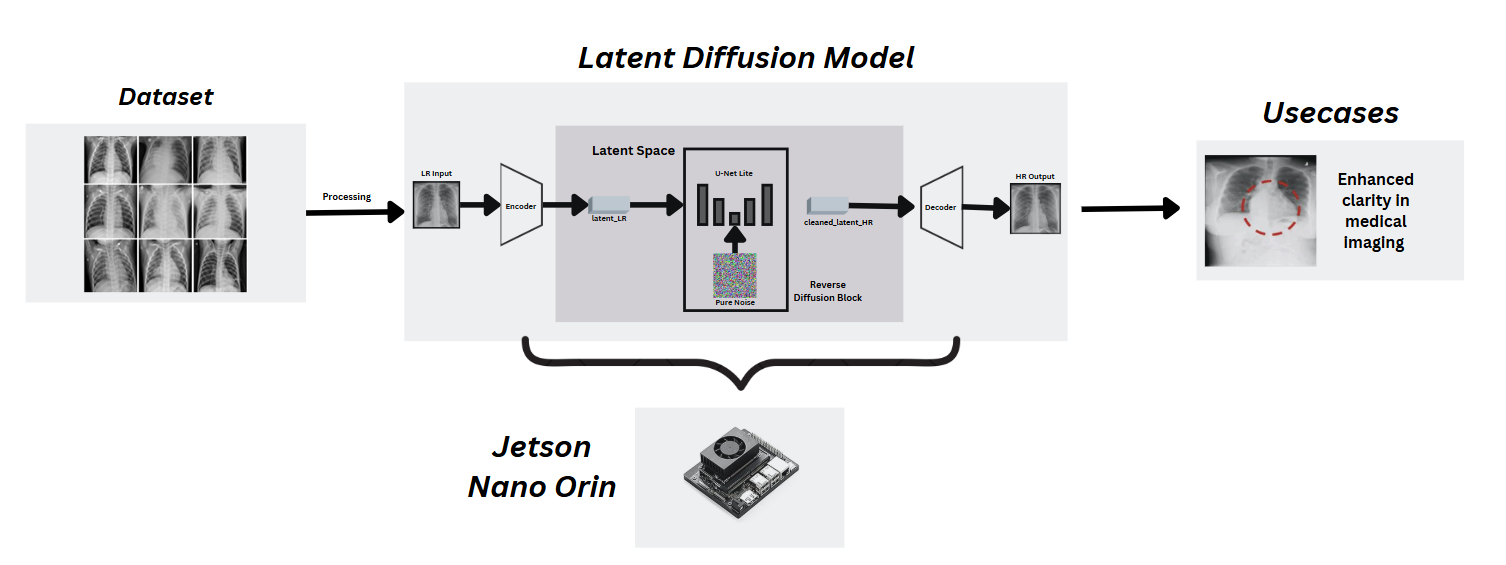
\includegraphics[width=0.9\textwidth]{progress/Figs/modelmain.png}
\end{center}
\caption{The proposed model.}
\label{modelmain}
\end{figure}

\section{Background And Related Work}

\subsection{A Brief History of Super Resolution (SR)}

Super-resolution (SR) is the task of reconstructing high-resolution (HR) images from low-resolution (LR) counterparts. Early SR methods predominantly used traditional interpolation techniques such as bicubic interpolation, where weighted averages of surrounding pixels approximate unknown pixel values. This general-purpose resampling method works for both upsampling and downsampling but cannot capture fine detail and often introduces blur, as explained by the Data Processing Inequality, which states that information not present in the original image cannot be created \citep{cover2012elements}. As a result, there have been recent shifts to exploring Deep Neural Network based frameworks as a means to inject learned information from the Neural Networks, into low-resolution images in order to increase resolution in a manner that actually adds informative content.

Deep learning brought major advances, starting with SRCNN \citep{dong2015cnn}, which used convolutional neural networks (CNNs) to outperform traditional methods in PSNR. These CNN models, however, relied on pixel-wise losses (L1, L2) that often produced overly smooth outputs. SRGAN \citep{ledig2017gan} addressed this by introducing adversarial training to improve perceptual quality, and ESRGAN \citep{wang2018esrgan} further enhanced GAN stability and depth. Despite these gains, GAN-based SR remains challenging due to the delicate balance required between generator and discriminator for stable convergence.

U-Net \citep{ronneberger2015unet}, originally for biomedical segmentation, became a popular backbone for image-to-image tasks. Its encoder–decoder with skip connections preserves fine detail while capturing global context, but operating in pixel space makes it memory-intensive, slow to train, and unsuitable for edge devices.

Latent Diffusion Models (LDMs) \citep{rombach2022latent} address these limitations by performing the diffusion process in a low-dimensional latent space produced by a Variational Autoencoder. This reduces the spatial size of U-Net inputs, lowering computation and memory costs while enabling state-of-the-art results in systems like Stable Diffusion. Recent work, such as Edge-SD-SR \citep{mehdi2025edgesd}, demonstrates that latent diffusion-based SR can run efficiently on mobile and edge devices, greatly reducing model size and latency without compromising output quality.

\subsection{Evaluation Metrics in Super-Resolution}

Super-resolution quality is evaluated using Peak Signal-to-Noise Ratio (PSNR), Structural Similarity Index Measure (SSIM), and Learned Perceptual Image Patch Similarity (LPIPS). PSNR quantifies pixel-wise differences between reconstructed and reference images, while SSIM measures structural similarity \citep{huynh2008scope, wang2004image}. LPIPS \citep{zhang2018lpips} assesses perceptual similarity using deep features extracted from pretrained convolutional neural networks, capturing high-frequency details and aligning better with human perceptual judgment than PSNR or SSIM. 

\section{Data Processing}

The dataset used is the publicly available NIH ChestX-ray14 dataset \citep{wang17} consisting of 112,120 1024x1024 images of chest X-rays from 30,805 unique patients.

The Indiana University Chest X-Ray Collection of more than 7000 images accessible through Open-i \citep{demner2016} is used as additional testing data. It contains both lateral and frontal view X-rays, as opposed to the NIH set which contains only frontal X-rays. This will ensure that the model can be tested on images completely different from its training data.

\subsection{Data Loading}

The following steps were used to obtain and process the dataset, of which a few sample images are shown in Figure~\ref{training_samples}:

\begin{enumerate}
    \item \textbf{Data downloading and organization:} A downloading script allows the user to download a specified number of batches from the dataset source, extracts them into the specified folder, and prevents overwriting of existing data.
    
    \item \textbf{Generating HR and LR image pairs:} The \texttt{generate\_downsampled\_pairs} function downsamples the original 1024x1024 images twice using OpenCV’s \texttt{resize} function with bicubic interpolation. The 256x256 downsampled image is saved into the \texttt{HR\_256} folder and the 64x64 version is saved into the \texttt{LR\_64} folder.
    
    \item \textbf{Creating a custom PyTorch dataset:} The \texttt{PairDataset} class reads images from their folders, transforms them into tensors of type \texttt{float32} and normalizes them to [-1,1] for faster training convergence. It assembles mini-batches of dimension B$\times$3$\times$64$\times$64 or B$\times$3$\times$256$\times$256 for input images and labels (ground truths) respectively.
    
    \item \textbf{Dataset splitting:} The \texttt{PairDataset} class also allows for configurable splits between train/validation/test data. A 70-20-10 split is currently in use, which provides 38,527 training, 10,907 validation, and 5,500 test images. One of the challenges here was to keep images from the same patient together, which was solved using careful parsing of filename while generating split indices.
\end{enumerate}

The same steps will be followed for testing on the new data (Indiana University). The only required change will be to set the data directory (a configurable argument) to the directory where the new data has been extracted, and to ensure images are cropped to squares before resizing.

\begin{figure}[h]
\begin{center}
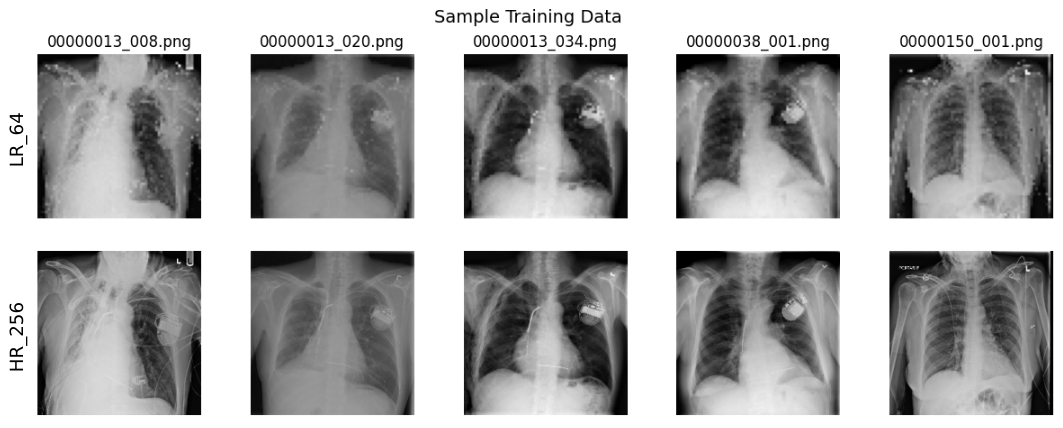
\includegraphics[width=1\textwidth]{Figs/training_samples.png}
\end{center}
\caption{Some random samples of the training data without data augmentation.}
\label{training_samples}
\end{figure}

\subsection{Data Augmentation}

To improve generalization and robustness, data augmentation was applied to 70\% of the training samples. This percentage was chosen based on empirical studies suggesting that moderate augmentation (around 60--80\%) helps prevent overfitting while maintaining data fidelity, which is particularly important in the medical imaging domain where fine-grained details are critical \citep{athalye23, sanaat22}. Each augmentation was implemented considering spatial alignment, ensuring that LR and HR image pairs remained synchronized. The augmentation techniques used are as follows:

\begin{itemize}
    \item \textbf{Random Horizontal Flip (50\%):} Flips images along the vertical axis to make the model invariant to left-right orientation.
    \item \textbf{Random Rotation (90°, 180°, 270°):} Simulates different acquisition angles while preserving anatomical structure.
    \item \textbf{Random Resized Crop (80\%):} Crops and resizes the image to expose subregions, helping the model detect abnormalities anywhere in the X-ray.
    \item \textbf{Cutout (30\%):} Masks a 20\% square patch to simulate occlusions or artifacts, encouraging the model to rely on surrounding context.
\end{itemize}

Demonstrations of these augmentations are shown in Figure~\ref{augmentations}.

While implementing these techniques, care was taken to maintain alignment between LR and HR image pairs, particularly during cropping, which required scaling coordinates appropriately. Unrealistic augmentations such as color jitter or geometric warping were avoided to preserve the medical validity of the X-rays. Applying augmentation to roughly 70\% of the training data balanced introducing useful variation with retaining enough original examples for accurate learning.

\begin{figure}[h!]
\centering
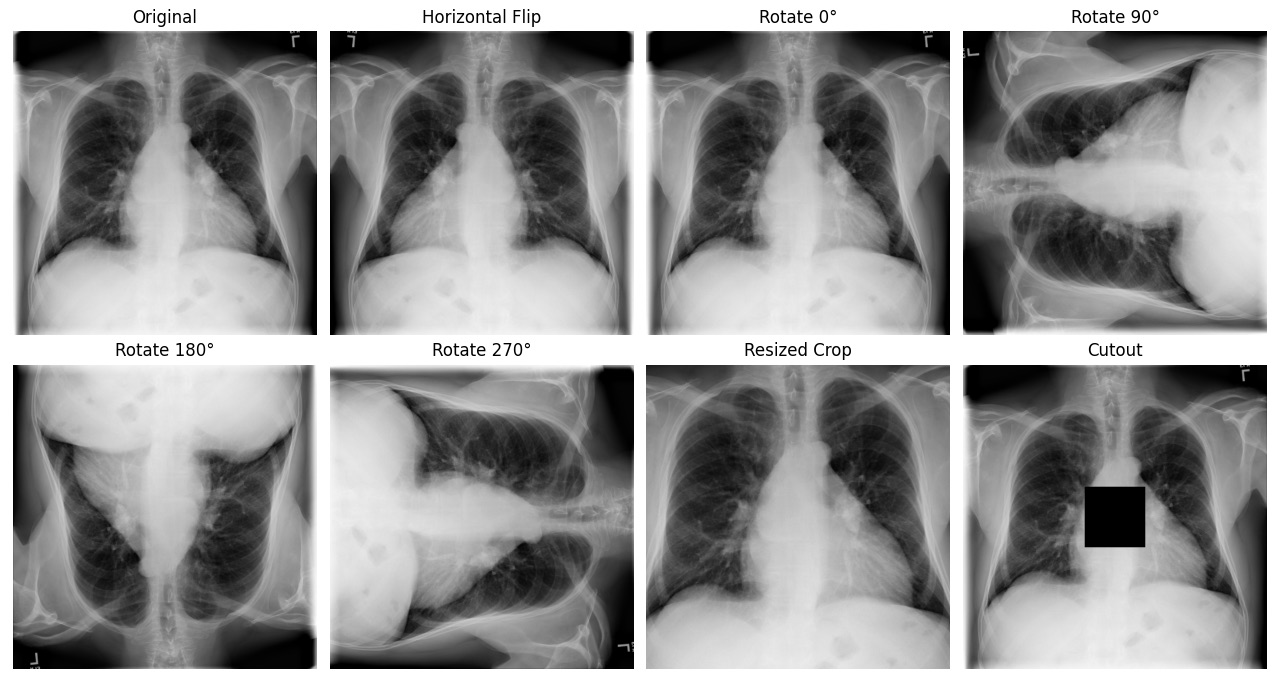
\includegraphics[width=0.8\textwidth]{Figs/augmentation.jpg}
\caption{Demonstration of augmentation techniques used in model training.}
\label{augmentations}
\end{figure}

\section{Architecture}

The primary model performs super-resolution on low-resolution chest X-rays using a latent diffusion-based architecture. As shown in Figure~\ref{model2}, the system includes a pretrained VAE, custom diffusion schedulers, and a custom U-Net, totaling 813,220 trainable parameters. All training and inference was conducted on an NVIDIA GeForce RTX 4090.

\begin{figure}[h]
\begin{center}
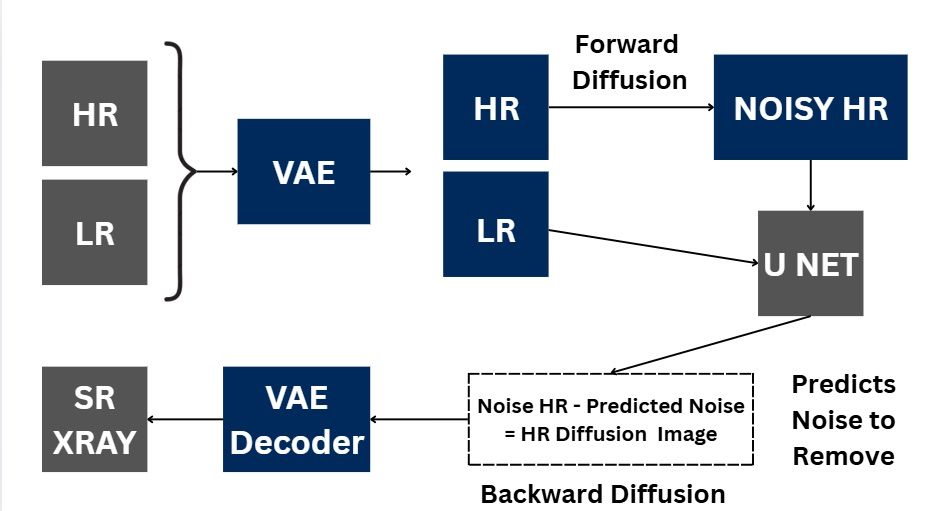
\includegraphics[width=0.7\textwidth]{progress/Figs/model2.jpg}
\end{center}
\caption{High level block diagram of architecture used for both training and inference.}
\label{model2}
\end{figure}

\subsection{Latent Diffusion-Based Super-Resolution}

The model takes paired LR and HR images (3×64×64 and 3×256×256). LR images are first upsampled to 3×256×256 via bicubic interpolation, then both LR and HR images are encoded to latent space separately using Hugging Face’s pretrained AutoencoderKL VAE, yielding 4×32×32 latents by reducing spatial resolution 8× and expanding channels from 3 to 4.

\subsection{Forward Diffusion and Timestep Conditioning}

Training uses the forward diffusion process, where Gaussian noise is progressively added to the HR latent over multiple time steps. Rather than sequentially applying noise at each step, we use the closed-form DDPM formula for efficiency:
\[
z_t = \sqrt{\bar{\alpha}_t} \cdot z_0 + \sqrt{1 - \bar{\alpha}_t} \cdot \epsilon
\]
This closed form calculates the final noisy HR latent given some number of timesteps \( t \in [0, 300) \). The timestep \( t \) controls the noise level, as a higher \( t \) implies more steps that add noise. \( z_0 \) is the clean HR latent, \( \epsilon \sim \mathcal{N}(0, 1) \), and
\[
\bar{\alpha}_t = \prod_{i=1}^{t} (1 - \beta_i)
\]
with \( \beta \) linearly scheduled from 0.0001 to 0.02, as per the original DDPM paper \citep{ho20}. The noisy HR latent is concatenated with the LR latent to form an 8-channel tensor passed to the U-Net, alongside the timestep \( t \).

U-Net uses an encoder-decoder structure with skip connections (Figure~\ref{model3}) \citep{ronneberger2015unet}. Through conditioning available from the LR latent and \( t \), the U-Net learns to predict the noise added to the HR latent, trained using LPIPS loss against the true \( \epsilon \) added during the forward diffusion process.

\begin{figure}[h]
\begin{center}
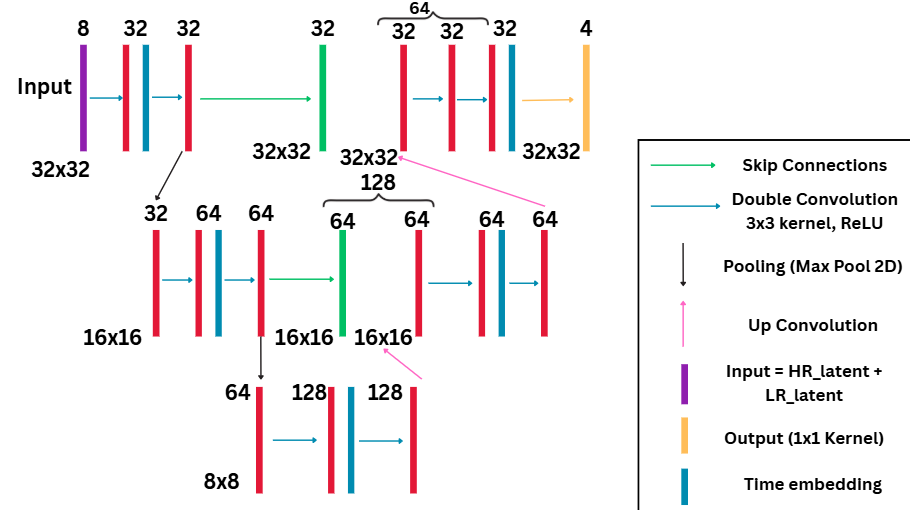
\includegraphics[width=0.9\textwidth]{progress/Figs/model3.png}
\end{center}
\caption{Structure of the U-Net.}
\label{model3}
\end{figure}

\subsection{Inference and Reverse Diffusion}

During inference, the process starts from pure Gaussian noise in latent space (\(4 \times 32 \times 32\)). Reverse diffusion is performed from \( t = 299 \) to \( 0 \), iteratively denoising with the trained U-Net. At each step, the LR latent is concatenated with the noisy HR latent, and the predicted \( \hat{\epsilon}_t \) is used to reverse the noise. After all steps, the final latent is decoded via the VAE to produce a \(3 \times 256 \times 256\) super-resolved image. PSNR, SSIM and LPIPS are used to measure performance against ground-truth HR images, with bicubic interpolation as the baseline.

\subsection{Edge Deployment for Performance Boost}

To accelerate inference and prepare the model for deployment on resource-constrained edge devices, we optimized the trained U-Net using NVIDIA TensorRT. After training, the PyTorch checkpoint (\texttt{.pt}) containing only the U-Net weights was exported to the ONNX format (\texttt{.onnx}) using \texttt{torch.onnx.export}, preserving the same input-output interface (x: 8×32×32, t: scalar timestep). The ONNX model was then compiled into a TensorRT engine file (\texttt{.trt}) using \texttt{trtexec}, TensorRT’s command-line compiler.

During inference, the TensorRT runtime loads the optimized engine, allocates GPU and CPU buffers, and executes inference using an asynchronous CUDA stream. The LR and noisy HR latents are flattened into contiguous NumPy arrays and copied to GPU memory, where the U-Net performs a forward pass to predict noise. The resulting output is transferred back to CPU memory and reshaped into the original latent format.


\section{Baseline Model}

A bicubic interpolation algorithm \citep{keys1981cubic} is used as the baseline model. The input LR image is resized to an HR image via PyTorch's \texttt{F.interpolate} function with \texttt{mode='bicubic'} and \texttt{align\_corners=False} parameters. Bicubic interpolation is widely used in image processing due to its computational efficiency and smooth results, though it cannot recover high-frequency details lost during downsampling.

\section{Quantitative Results}

The dataset was split into 70\% train, 20\% validation, and 10\% test. Training ran for 50 epochs, and all twelve available training batches were loaded. Both training and validation losses dropped smoothly to about 0.18 (Figure~\ref{v1loss}). Evaluation was performed on the NIH ChestX-ray14 patient-held-out test split, computing PSNR, SSIM, and LPIPS on images and reporting the means over all samples in the test set. Bicubic interpolation serves as a non-learned baseline. Higher is better for PSNR/SSIM and lower is better for LPIPS. The latent-diffusion model achieved PSNR/SSIM values that are slightly lower than bicubic but still comparable, while achieving substantially lower LPIPS (Table~\ref{tab:sr_results}). These results indicate greater perceptual similarity but slightly degraded pixel-wise similarity.

On the test set, the TensorRT-optimized U-Net reduced inference time, achieving a 4.7$\times$ speedup compared to the standard PyTorch model. PSNR, SSIM, and LPIPS remained within negligible differences, indicating that the performance gains came without meaningful loss in image quality.

\begin{figure}[h]
\begin{center}
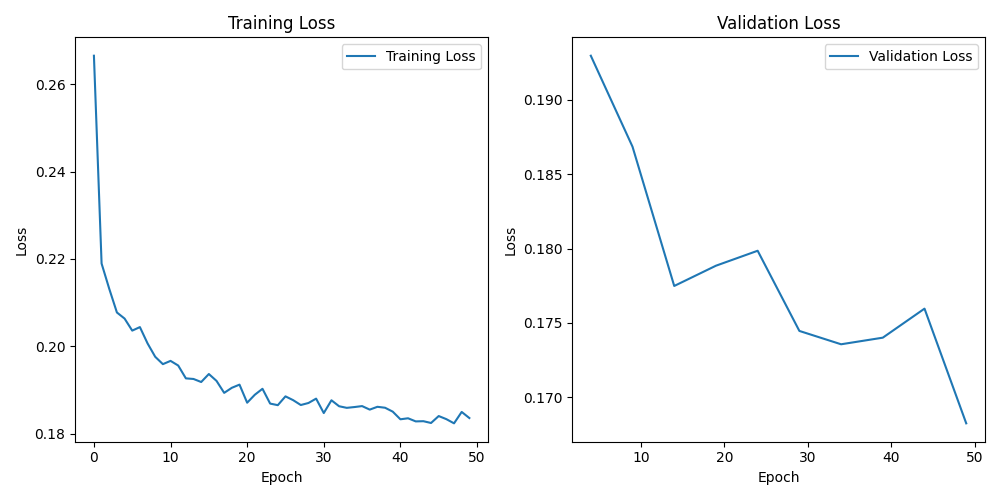
\includegraphics[width=0.8\textwidth]{progress/Figs/trainv1loss.png}
\end{center}
\caption{Training and validation curves.}
\label{v1loss}
\end{figure}

% Increase row height slightly
\renewcommand{\arraystretch}{1.3}

\begin{table}[h!]
\centering
\caption{Inference time and quality metrics for bicubic, diffusion, and TensorRT models. Lower LPIPS is better, while higher PSNR/SSIM are better.}
\label{tab:sr_results}
\begin{tabular}{l c c c c c}
\toprule
\textbf{Inference Type} & 
\textbf{Time} & 
\textbf{Model} & 
\textbf{LPIPS} & 
\textbf{PSNR} & 
\textbf{SSIM} \\
\midrule
N/A        & N/A   & Bicubic   & 0.3472 & 29.59 & 0.9176 \\
Standard   & 7.02s & Diffusion & 0.1232 & 27.34 & 0.8647 \\
TensorRT   & 1.49s & Diffusion & 0.1223 & 27.11 & 0.8501 \\
\bottomrule
\end{tabular}
\end{table}

\section{Qualitative Results}

Figure~\ref{val_samples} compares two test samples across LR (64$\times$64), bicubic (256$\times$256), diffusion SR (256$\times$256), and HR (256$\times$256). Diffusion SR yields sharper bone edges, clearer diaphragm contours, and finer lung textures than bicubic, aligning with its lower LPIPS despite slightly lower PSNR/SSIM. The model struggles with distortions, artifacts, or text in LR inputs, sometimes smoothing or hallucinating details. For example, the white `L' marker above the right shoulder in the bottom-right HR image is blurred in the diffusion output. Ribs also appear slightly less pronounced than in HR, though still more accurate than bicubic.

\begin{figure}[h]
\begin{center}
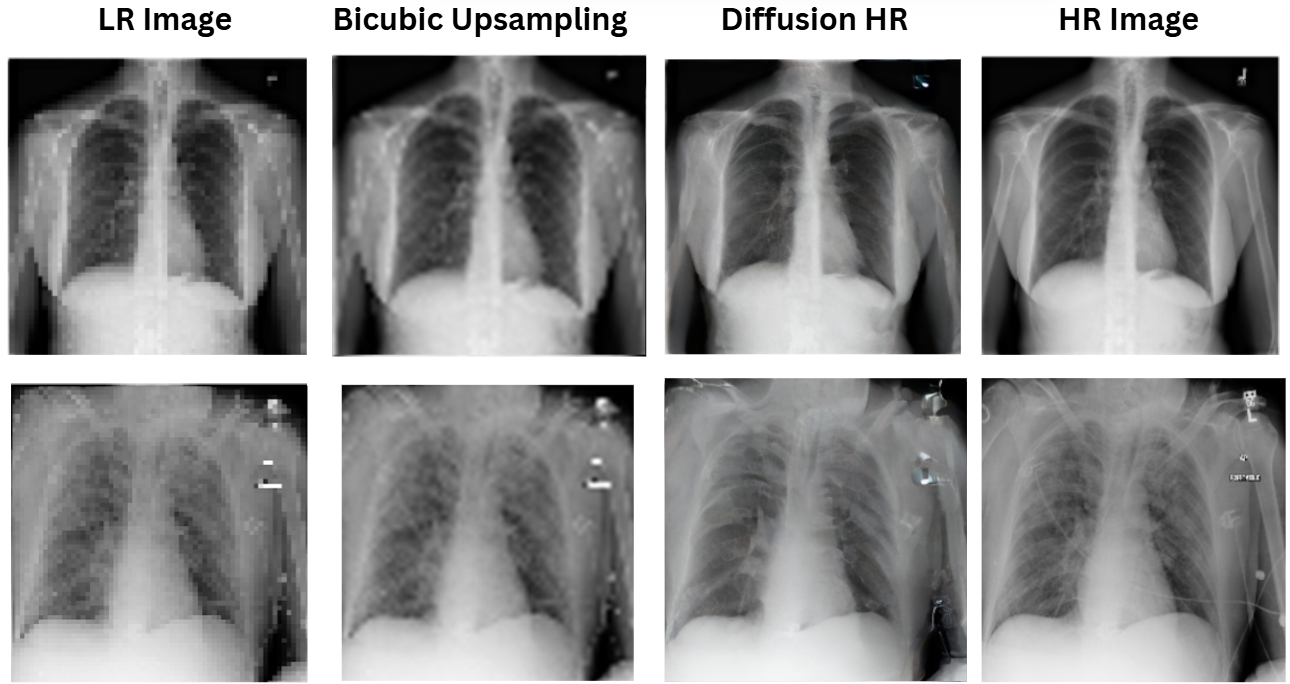
\includegraphics[width=0.7\textwidth]{progress/Figs/val_samples.png}
\end{center}
\caption{Sample results using test data.}
\label{val_samples}
\end{figure}

TensorRT outputs were nearly identical to PyTorch, with only slight contrast/sharpness differences in fine structures, thus matching the small PSNR changes (Figure~\ref{tensor_val}). A subtle tendency was observed for TensorRT outputs to produce slightly darker regions in already dark areas of the image.

\begin{figure}[h]
\begin{center}
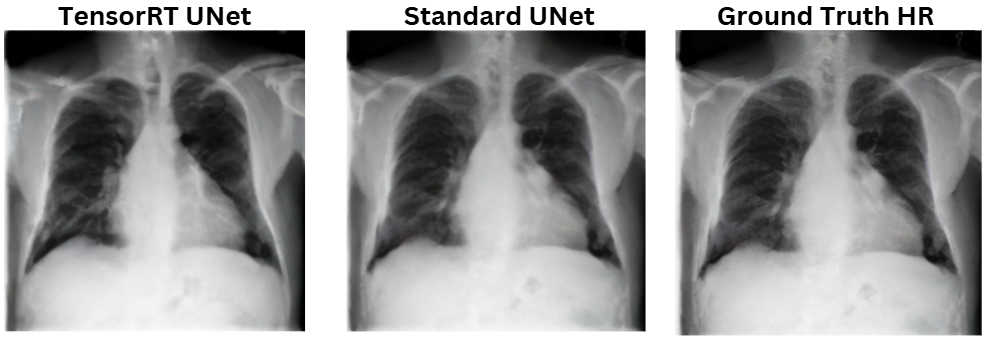
\includegraphics[width=0.6\textwidth]{progress/Figs/tensor_val.png}
\end{center}
\caption{Comparison of model with TensorRT on test set.}
\label{tensor_val}
\end{figure}

\section{Evaluation of model on new data}

% Increase row height slightly
\renewcommand{\arraystretch}{1.3}

The model was trained exclusively on the NIH ChestX-ray14 dataset. To assess true generalization, the model was tested on the Indiana University Chest X-Ray Collection which is a fully independent frontal chest x-ray dataset sourced from a different institution with no shared images. The Indiana Collection introduces imaging conditions not present during training, thus challenging the model’s adaptability. Its independent origin ensures that these test samples were not used in any training or tuning of hyperparameters, providing a clean, unbiased evaluation of performance on new data.

On the unseen data, the latent diffusion model performed similarly to the NIH dataset, clearly outperforming bicubic by recovering fine anatomical details and diagnostic features lost with traditional methods (Figure~\ref{test_samples}), though it still hallucinated fine text, noise, and artifacts.

Means for metrics on the Indiana dataset closely matched the means for metrics on the NIH dataset, with PSNR/SSIM slightly lower and LPIPS showing a significant improvement (Table~\ref{tab:test_results}).

\begin{figure}[h]
\begin{center}
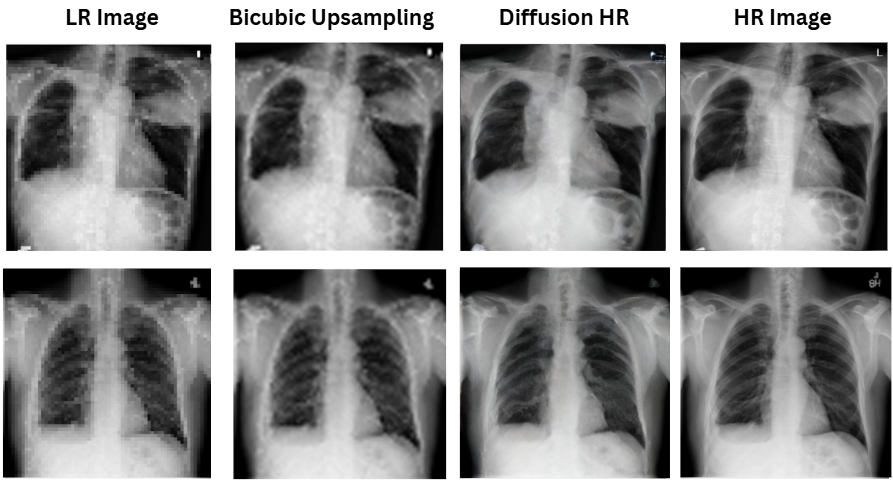
\includegraphics[width=0.7\textwidth]{progress/Figs/test_samples.png}
\end{center}
\caption{Sample results using unseen new data.}
\label{test_samples}
\end{figure}

\begin{table}[h]
\centering
\caption{Inference time and quality metrics on the unseen new data for bicubic, diffusion, and TensorRT models. Lower LPIPS is better, while higher PSNR/SSIM are better.}
\label{tab:test_results}
\begin{tabular}{l c c c c c}
\toprule
\textbf{Inference Type} & 
\textbf{Time} & 
\textbf{Model} & 
\textbf{LPIPS} & 
\textbf{PSNR} & 
\textbf{SSIM} \\
\midrule
N/A        & N/A   & Bicubic   & 0.3444 & 28.36 & 0.9019 \\
Standard   & 7.11s & Diffusion & 0.1285 & 26.74 & 0.8621 \\
TensorRT   & 1.70s & Diffusion & 0.1290 & 27.01 & 0.8280 \\
\bottomrule
\end{tabular}
\end{table}

The TensorRT-optimized U-Net reduced inference time, achieving a similar 4.2$\times$ speedup compared to the standard PyTorch model. This improvement is similar to that of the NIH results and it was expected, as runtime depends on model architecture and TensorRT’s optimizations rather than the specific dataset. Output quality remained comparable, with only minor contrast differences as noted in the validation results (Figure~\ref{tensor_test}).

\begin{figure}[h]
\begin{center}
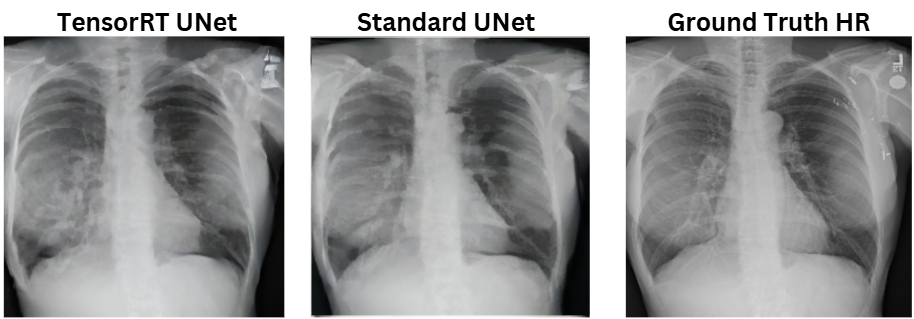
\includegraphics[width=0.6\textwidth]{progress/Figs/tensor_test.png}
\end{center}
\caption{Comparison of model with TensorRT on unseen new data.}
\label{tensor_test}
\end{figure}

\section{Discussion}

The latent-diffusion SR produces chest X-rays that are perceptually closer to the HR targets than bicubic, as seen by richer rib edges, diaphragm contour, and textures. This aligns with lower LPIPS even when PSNR/SSIM are similar or slightly lower. This is expected since after downsampling, the LR image has lost high-frequency content. A linear interpolator like bicubic can only smooth between existing samples and so it could not recover lost high-frequency information. Diffusion, by contrast, used a learned prior over HR chest X-rays and estimates samples from the conditional distribution $p(\mathrm{HR} \mid \mathrm{LR})$, thus synthesizing a brand new image from noise. That prior injected high-frequency details (edges/texture) that are consistent with the LR evidence, as opposed to simply smoothing from existing samples. Because many HR images are plausible for the same LR input, a pixel-wise metric could penalize these valid choices, explaining why perceptual quality improves (LPIPS) while PSNR/SSIM may not.

Looking at the qualitative results, the shortcomings arise when non-anatomical artifacts (compression blockiness, clipped borders, markers) are present. In these cases, the model may smooth or invent details, as visible around borders and in regions with distortions/unnatural noise. Additionally, thin, high-contrast anatomy such as the clavicles and ribs appeared slightly faint, perhaps due to the VAE bottlenecking very thin edges and/or pre-encoding upsample adds blur which the model does not always fully reverse. A somewhat surprising finding was how strongly LPIPS improved even when PSNR/SSIM slightly dipped, highlighting that pixel-aligned metrics can undervalue clinically reasonable reconstructions.

For deployment on resource-constrained hardware, the observed inference speedup from TensorRT stems from kernel fusion, reduced precision operations, and hardware-specific optimizations that lower computational overhead. The slight quality degradation likely results from quantization and approximation during these optimizations, which can slightly affect fine-scale contrast and edge definition.

Overall, the model's strengths are perceptual realism and anatomical accuracy under typical conditions. Conditioning in latent space keeps global structure anchored while the denoiser invents plausible high-frequency detail. The TensorRT export also delivered a meaningful speedup with only minor, mostly contrast-level differences, suggesting practicality for edge deployment.

Key challenges involved designing and integrating the diffusion scheduler with the VAE and U-Net. As a latent diffusion model, the system required a solid understanding of discrete-time stochastic processes and variational inference to generate images from pure noise. A significant portion of time was spent reading relevant literature and working through the underlying math to ensure correct implementation. Another key challenge was sourcing the Jetson Nano. To address the observed artifact sensitivity and faint bones, we will scale and tune the system: train on the full dataset for a longer duration with larger effective batch sizes (feasible via gradient accumulation), adopt a deeper U-Net to address bottlenecks, and implement cross-attention between the LR and HR latents prior to entering the U-Net, instead of the current naive concatenation of feature vectors. Together, these steps should further elevate the perceptual gains into more reliable, clinically usable outputs.

\section{Ethical Considerations}

While promising for improving diagnostic support by enhancing low-resolution chest X-ray images, this system should be used with caution and further validated for safe, fair clinical use.
Public datasets, like the one being used for this project, usually lack demographic diversity, which risks bias and reduced performance on underrepresented populations \citep{Galanty2024BEAMRAD}. The diffusion-based architecture relies on generative modeling in a latent space, which sometimes introduces hallucinated details not present in the original scan. These enhancements must not be mistaken for real anatomical features, as they could mislead diagnoses if not carefully validated \citep{Shin2024SuperResolution}.

\clearpage

\label{last_page}

\bibliography{APS360_ref}
\bibliographystyle{iclr2022_conference}

\end{document}
